% Generated by julia/scripts/generate_figure_audit_artifacts.jl.
% Exact source: experiments/results/summaries/innovation_safe_bridge.csv.
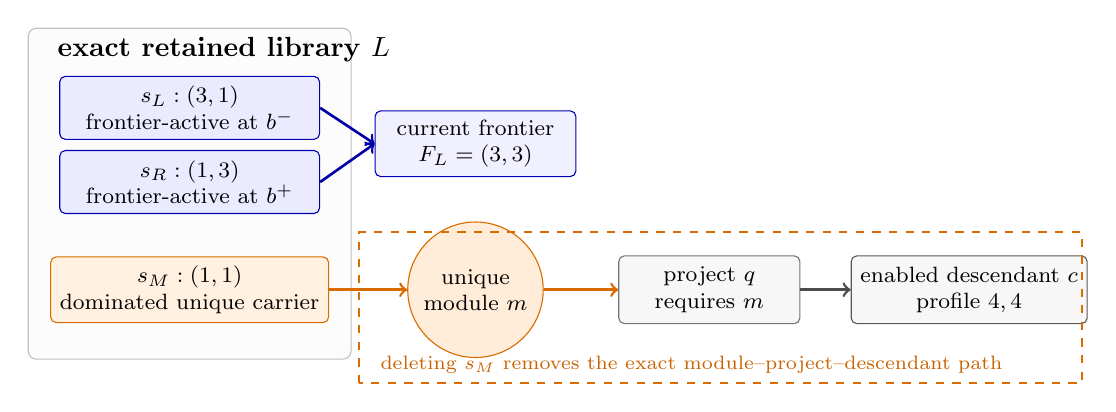
\begin{tikzpicture}[x=1cm,y=0.76cm,font=\footnotesize]
  \tikzset{
    active/.style={draw=blue!70!black,fill=blue!8,rounded corners=2pt,
      minimum width=3.30cm,minimum height=0.80cm,align=center},
    bridge/.style={draw=orange!85!black,fill=orange!12,rounded corners=2pt,
      minimum width=3.30cm,minimum height=0.80cm,align=center},
    module/.style={draw=orange!85!black,fill=orange!15,circle,
      minimum size=1.20cm,align=center},
    project/.style={draw=black!55,fill=black!3,rounded corners=2pt,
      minimum width=2.30cm,minimum height=0.86cm,align=center},
    descendant/.style={draw=black!65,fill=black!3,rounded corners=2pt,
      minimum width=2.50cm,minimum height=0.86cm,align=center},
    flow/.style={->,line width=0.95pt,draw=black!70}
  }
  \draw[draw=black!25,rounded corners=3pt,fill=black!1]
    (-0.2,-0.78) rectangle (3.90,4.75);
  \node[font=\bfseries,anchor=west] at (0.05,4.40)
    {exact retained library \(L\)};

  \node[active] (left) at (1.85,3.42)
    {\(s_L:(3,1)\)\\frontier-active at \(b^-\)};
  \node[active] (right) at (1.85,2.18)
    {\(s_R:(1,3)\)\\frontier-active at \(b^+\)};
  \node[bridge] (bridge) at (1.85,0.38)
    {\(s_M:(1,1)\)\\dominated unique carrier};

  \node[draw=blue!70!black,fill=blue!6,rounded corners=2pt,
    minimum width=2.55cm,minimum height=0.80cm,align=center]
    (frontier) at (5.48,2.82) {current frontier\\\(F_L=(3,3)\)};
  \draw[flow,draw=blue!65!black] (left.east) -- (frontier.west);
  \draw[flow,draw=blue!65!black] (right.east) -- (frontier.west);

  \node[module] (module) at (5.48,0.38) {unique\\module \(m\)};
  \draw[flow,draw=orange!85!black] (bridge.east) -- (module.west);
  \node[project] (project) at (8.45,0.38) {project \(q\)\\requires \(m\)};
  \draw[flow,draw=orange!85!black] (module.east) -- (project.west);
  \node[descendant] (descendant) at (11.75,0.38)
    {enabled descendant \(c\)\\profile \(4,4\)};
  \draw[flow] (project.east) -- (descendant.west);

  \draw[dashed,orange!85!black,line width=0.85pt]
    (4.00,-1.18) rectangle (13.18,1.34);
  \node[anchor=west,text=orange!78!black,font=\scriptsize] at (4.15,-0.87)
    {deleting \(s_M\) removes the exact module--project--descendant path};
\end{tikzpicture}
